\subsection{Candidate Models}
Given the baseline performance of the pretrained VGG16 with places image preprocessing, a set of candidate models are proposed with the aim of 1) improving accuracy and 2) reducing dimensionality of feature vectors allowing for faster computation of similarity matrix.
The results from \autoref{sec:baselinemodels} would suggest, that out-of-the-box performance for autoencoder arhcitectures may perform better in producing well-defined encodings from VGG16's fc\_1-layer using Places image preprocessing. 

\paragraph{Pretrained Model with Denoising Autoencoder} \\~
Several configurations of pretrained models with denoising autoencoders have been attempted throughout experimentation. 
Generally autoencoders in this setting tend to perform better when the first encoder layer is of similar dimensions to the input feature vector. 
Broader bottlenecks also tend to retain more information during training. 

\begin{table}[H]
  \centering
  \resizebox{\textwidth}{!}{%
  \begin{tabular}{llllllll}
  \hline
  Pretrained    & AE Layers                   & Preprocessing   & Test Acc.      & Val. Acc.      & Top-5 Test Acc. & Top-5 Val. Acc. \\ \midrule
  ResNet50 (max\_pool) & 2048, 512    & Simple              & 0.337          & 0.338          & 0.693           & 0.697           \\
  ResNet50 (max\_pool) & 2048, 512    & ImageNet           & 0.341          & 0.328          & 0.704           & 0.671           \\
  ResNet50 (max\_pool) & 2048, 512    & Places             & 0.650          & 0.661          & \textbf{0.927}  & 0.911           \\
  VGG16 (fc\_1)        & 4096, 1028   & Simple              & 0.528          & 0.529          & 0.818           & 0.820           \\
  VGG16 (fc\_1)        & 4096, 1028   & Places              & \textbf{0.778} & \textbf{0.783} & 0.915           & \textbf{0.928}  \\ \bottomrule
  \end{tabular}%
  }
  \catption{Initial experiments with denoising autoencoders, noise-factor = 0.3}
  \label{tab:daeresults}
\end{table}

It would appear, that models trained on input preprocessed with Simple or ImageNet prepocessing schemes achieve significantly lower accuracies compared to models trained on Places preprocessed data. 
Furthermore, models with Places pretrained weights perform better across the board, all else equal. 


\paragraph{Pretrained Model with Deep Autoencoder} \\~
Initial experiments with deep autoencoders show no significant boosts to performance in using either ResNet50 or VGG16 compared to the denoising counterparts. 
\begin{table}[H]
  \centering
  \resizebox{\textwidth}{!}{%
  \begin{tabular}{@{}llllllll@{}}
  \toprule
  Pretrained    & AE Layers                   & Preprocessing   & Test Acc.      & Val. Acc.      & Top-5 Test Acc. & Top-5 Val. Acc. \\ \midrule
  ResNet50      & 2048, 1028, 512             & Simple          & 0.324          & 0.345          & 0.698           & 0.664           \\
  ResNet50      & 2048, 1028, 512             & Places          & 0.659          & 0.654          & \textbf{0.926}  & 0.929           \\
  VGG16         & 4096, 2048, 1028            & Simple          & 0.541          & 0.516          & 0.830           & 0.820           \\
  VGG16         & 4096, 2048, 1028            & Places          & \textbf{0.775} & \textbf{0.764} & 0.914           & \textbf{0.934}  \\
  VGG16         & 6000, 4000, 3000, 2000, 800 & Places          & 0.745          & 0.749          & 0.9             & 0.915           \\ \bottomrule
  \end{tabular}%
  }
  \catption{Initial experiments with deep autoencoders}
\end{table}
Deep autoencoders can be said to perform on-par with narrower denoising autoencoders. They do however take longer to converge; see \autoref{appendix: D}. 

\paragraph{Pretrained Model with Deep Denoising Autoencoder} \\~
Adding noise to deep autoencoders yields slightly worse results in terms of accuracy compared to any of the previous approaches. 

\begin{table}[H]
  \centering
  \resizebox{\textwidth}{!}{%
  \begin{tabular}{@{}llllllll@{}}
  \toprule
  Pretrained   & Architecture     & Noise & Preprocessing & Test Acc.      & Val. Acc.      & Top-5 Test Acc. & Top-5 Val. Acc. \\ \midrule
  VGG16 & 4096, 2048, 1028 & 0.3   & Places        & \textbf{0.764} & \textbf{0.753} & \textbf{0.919}  & \textbf{0.913}  \\
  VGG16 & 4096, 2048, 1028 & 0.5   & Places        & 0.74           & 0.735          & 0.908           & 0.904          
  \end{tabular}%
  }
\end{table}
More results for DDAE's with pretrained layer alternation can be found in \autoref{appendix: C}.

\paragraph{Pretrained Model with Autoencoder} \\~
In later experiments it was shown, that the best candidate model was obtained by not using more sophisticated autoencoder architectures, but that shallow autoencoders without noise outperformed every other model and the baseline.




\subsection{Model Evaluation}
In the above section, minute improvements over the best baseline model were observed. 
This section produces a more in-depth, side-by-side comparison of the best-performing candidate model, in terms of test/val accuracy.
The shallow AE with Places image preprocessing from \autoref{tab:daeresults} achieves the best results among all candidate models. 
Furthermore, it outperforms the baseline on every metric.

\begin{figure}[H]
  \centering
    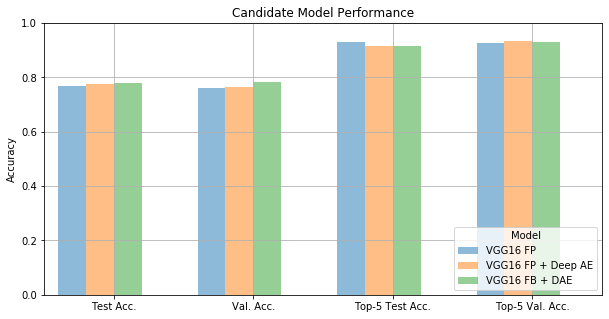
\includegraphics[width=\textwidth]{pictures/plots/candidate_acc}
    \caption{Candidate Model Accuracies v. Baseline}
    \label{fig:candidates}
\end{figure}

\subsubsection{Model Predictions}
The best DAE model, appears to have grasped very detailed image features in a feature vector smaller by factor \sfrac{1}{4} compared to the VGG16(fc\_1) forward passes.

\begin{figure}[H]
  \centering
    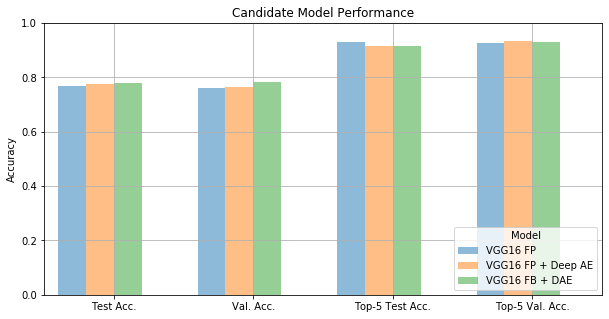
\includegraphics[width=\textwidth]{pictures/plots/candidate_acc}
    \caption{Candidate Model Accuracies v. Baseline}
    \label{fig:candidates}
\end{figure}


In order to get and understanding of the models it useful to map the feature vectors of a model into a 2-dimensional space using \texttt{t-SNE}\autocite{Chu2017}\autocite{HintonScience2006}. 
As suggested in \autocite{wattenberg2016how}, several combinations of hyperparameters were tested on train, test, and validation data; see \nameref{appendix: E}.
For all configurations, the DAE produces a lower KL-divergence, indicating that the DAE has learned a representation better at separating images that would otherwise be clumped together.

\begin{figure}[H]
    \centering
    \begin{subfigure}[b]{0.45\textwidth}
      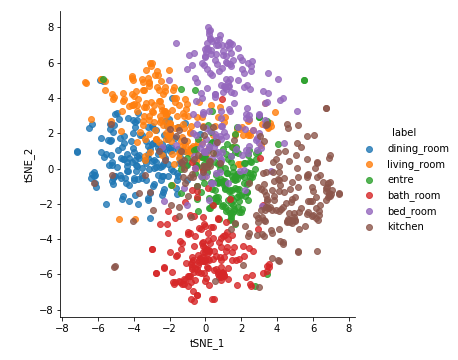
\includegraphics[width=\textwidth]{pictures/plots/tsne_vgg16}
      \caption{t-SNE: VGG16 Forward Pass, p=50}
      \label{fig:tsne1}
    \end{subfigure}
    %
    \begin{subfigure}[b]{0.45\textwidth}
      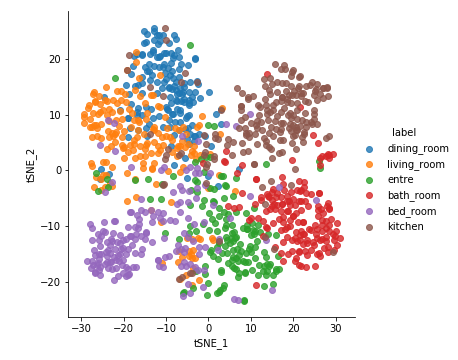
\includegraphics[width=\textwidth]{pictures/plots/tsne_vgg16_dae}
      \caption{t-SNE: VGG16 + Autoencoder,  p=50}
      \label{fig:tsne2}
    \end{subfigure}
    \caption{t-SNE feature space comparison}
    \label{fig:tsne}
\end{figure}



% \subsubsection{The Baseline Classification Accuracy}
% In determining the baseline accuracy score with which to compare candidate models with, two baselines have been tested - the one with higher accuracy serves as the baseline.

% \paragraph{A Vanilla Deep Denoising Autoencoder} ~\\
% The first candidate baseline model is a \texttt{Deep Denoising Autoencoder} trained on the images with only scaling applied as preprocessing steps.
% This network is a 150528, 512, 256, 128 autoencoder with noise added at the input layer. It also has regularization added at the bottleneck layer. 
% This modelling approach achieves a classification accuracy of 0.178.

% \paragraph{Forward Pass ResNet50 to MaxPool Layer} ~\\
% This baseline establishes the feasibility of simply passing information through ResNet50 pretrained on \texttt{ImageNet}. 
% This methodology achieves a classification accuracy of 0.161. 





% Model development was conducted by establishing a baseline model performance; this was done by establishing the class prediction accuracy of the ResNet50 model pre-trained on \textit{imagenet} data. 
% From then on, experimentation with more complicated model constructions was conducted:

% \begin{enumerate}
%     \item Baseline Deep Autoencoder without pretrained feature vectors from ResNet50
%     \item Deep Autoencoder with pretrained feature vectors from ResNet50
%     \item Deep Denoising Autoencoder with pretrained feature vectors from ResNet50
%     \item Deep Denoising Autoencoder with fine-tuned feature vectors from ResNet50
% \end{enumerate}

% \subsubsection{ResNet50 Feature Vectors}

% \subsubsection{Vanilla Deep Autoencoder}
% \subsubsection{Deep Autoencoder with pretrained feature vectors}
% \subsubsection{DDAE with pretrained feature vectors}
% \subsubsection{DDAE with fine-tuned feature vectors}

